\documentclass[main.tex]{subfiles}
\begin{document}
% FIXME FORMELN!
\chapter{Background}\label{chap:Background}
In this chapter, we present relevant literature needed to completely understand the proposed concept of \autoref{chap:Concept}.

\section{SLAM}
SLAM (Simultaneous Localization And Mapping) algorithms aim to solve a usual problem in the field of unmanned robotics;
A robot finds itself in an unknown environment and attempts to build a coherent map while keeping track of its location.
The robot uses use-case-specific sensors to obtain a snapshot of its current surroundings, which it then uses to update and enhance its known map (Mapping).
The robot then attempts to accurately estimate its position based on the updated map. The new information about its position is processed during the next map update.
Over decades of research, varieties of different (combinations of) sensors have been employed to solve this problem more accurately and efficiently.
Internal odometry sensors alone can be unreliable if the robot moves over uneven or slippery surfaces. For that reason, visual SLAM(V-SLAM) methods like \textit{MonoSLAM}\cite{1238654} or
\textit{Dense Visual SLAM}\cite{Kerl_Sturm_Cremers_2013} integrate additional visual input of camera sensors into their algorithm.
% FIXME elaborate
% FIXME Localization
% FIXME top-level Diagram!
% FIXME surveys!

\subsection*{RTAB-MAP}
RealSense-ROS internally uses a SLAM algorithm for map building, namely RTAB-MAP (Real-Time Appearance-Based Mapping)\cite{Labbé_Michaud_2019}.
Unlike purely visual-based SLAM algorithms, RTAB-MAP also takes input from odometry sensors, as well as an optional additional input in form of two- or three-dimensional
lidar scan.
% SECTION 
% FIXME "schon eher grob"
All these inputs are combined during a synchronization step, and the results thereof are passed to RTAB-MAP's \textit{Short-Term-Memory} (STM).
The STM assembles a new node from the new inputs and inserts it into the map graph. Based on the newly inserted node, RTAB-MAP attempts to determine if the current location has already been visited earlier, also known as \textit{loop closure}.
If a loop closure is detected, i.e., RTAB-MAP detects the re-visiting of a known location, the map graph is optimized and thus minimized. In addition, the global map is reassembled in correspondence with the new information.
The resulting map is published in the form of an unorganized point cloud.
% FIXME was ist der unterscheid zwischen OPC und UPC
% !SECTION
RTAB-MAP's general workflow is shown below in Figure~\ref{fig:rtabmap}:
% FIXME integrate figure into previous stanza
% FIXME why is the figure important
\begin{figure}[!h]
    \centering
    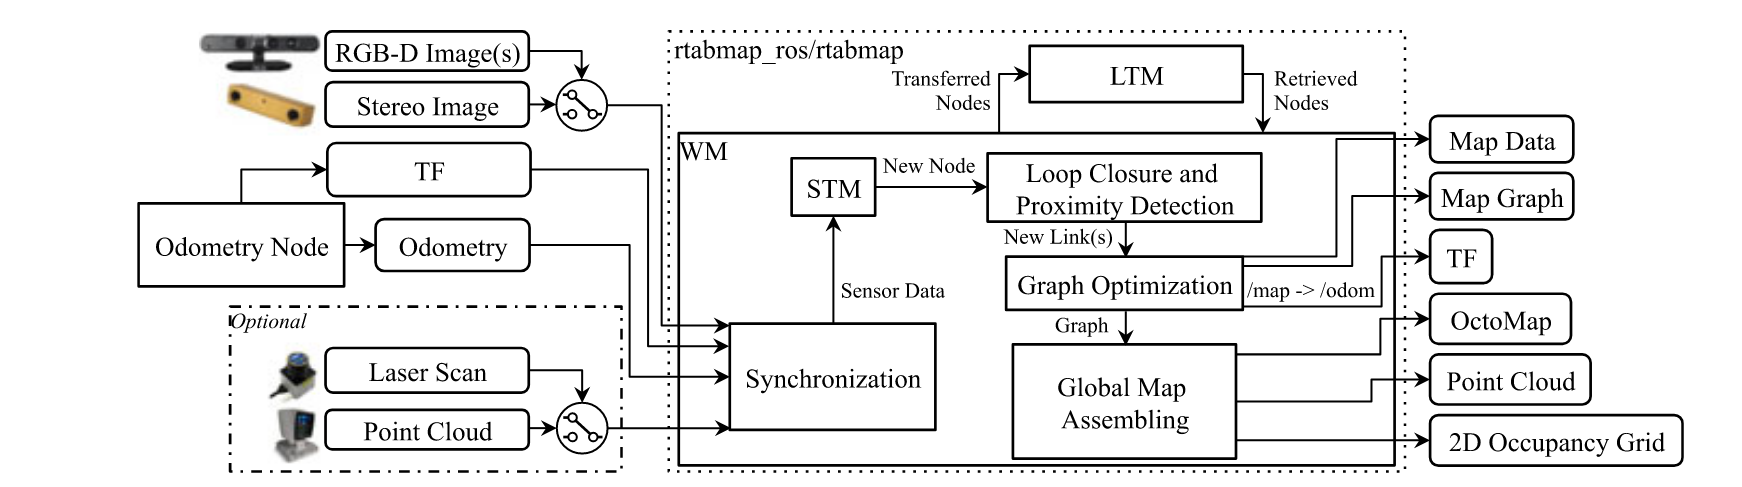
\includegraphics[width=15 cm]{images/rtabmap.png}
    \caption[RTAB-MAP Block Diagram]{Block diagram of RTAB-MAP's main node. Taken from \cite[Figure~1]{Labbé_Michaud_2019}}
    \label{fig:rtabmap}
\end{figure}

\section{Intel Realsense}
In this work, we use the Intel RealSense tracking camera T265 and the RGB-Depth(RGB-D) camera D455.
A tracking camera is generally used to observe the environment and usually has a wider field of view (FOV). The primary motivation for using RGB-D cameras is depth perception.
The primary differences and similarities between the T265 and the D455 are reported in Table~\ref{tab:cameraspecs}.
Beide Kameras sind stereo, die T265 hat 2 fisheye lenses und die D455 hat 2 imagers. Dazu hat die D455 noch einen RGB sensor und einen infrarot sensor. Mit dem IR sensor und den beiden imagern wird ein tiefenbild berechnet.
Durch die fisheye lenses hat die T265 mit 163° ein deutlich breiteres Sichtfeld  als die D455 mit nur 111°. Die maximale FPS anzahl der D455 ergibt sich aus den individuellen FPS werten der imager sensoren und dem RGB sensor, welche beide einen maximalwert von 90 haben.
Dazu sei gesagt, dass bei steigender auflösung die maximale Framerate sinkt und 90FPS nur mit einer maximalen auflösung von 640x480 möglich ist.
Furthermore, both cameras have an integrated Inertial Measurement Unit (IMU) which is used to compute its position in combination with visual input.
% FIXME explain tracking and RGB-D

Intel provides a software development kit, namely RealSense SDK, which allows easy and efficient use of the cameras.
The SDK runs on both Windows and Ubuntu, and a ROS(Robot Operating System \footnote{\href{https://www.ros.org/}{https://www.ros.org/}}) adaptation is also provided in Intel's Github repository \footnote{\href{https://github.com/IntelRealSense/realsense-ros}{https://github.com/IntelRealSense/realsense-ros}}.

\begin{table}[H]
    \centering
    \begin{tabular}{c|ccccccc}
             & Image  & Type     & max. Resolution & D-FOV & Shutter & Price & max. FPS \\ \hline
        D455 & Stereo & RGB-D    & 1280x720        & 111°  & global  & 419\$ & 90       \\ \hline
        T265 & Stereo & Tracking & 848 x 800       & 163°  & global  & 199\$ & 30
    \end{tabular}
    \caption[Intel RealSense T265 & D455 Specification]{Intel RealSense T265 and D455 camera specifications. More information and the complete Datasheets can be found on https://www.intelrealsense.com/.}
    \label{tab:cameraspecs}
\end{table}

\section{Plane Detection}

\paragraph*{introduction}
The field of plane detection has been around for decades. Most methods of detecting planar regions are based on one of three main categories \cite*{Limberger_Oliveira_2015,Araújo_Oliveira_2020}:
\begin{itemize}
    \item Hough Transform (HT)
    \item RANSAC (RC)
    \item Region Growing (RG)
\end{itemize}

\subsection*{Hough Transform}
The original motivation behind the Hough transform was detecting lines in images~\cite{5230799}. All points are sequentially processed via a voting procedure to detect the best fitting line over a set of 2d points.
Multiple lines with different orientations are fit through each given point $p$.
Because a line in slope-intercept form parallel to the y-axis would lead to an infinite slope, the Hesse normal form is chosen as the primary line representation\cite{10.1145/361237.361242}.

In Hesse normal form, an individual line can be parameterized with a pair $(r, \theta)$, with $r$  being the orthogonal distance origin to the plane and $\theta$ being the angle between the x-axis and the line that connects the origin to the closest point on the line.
This pair is also called a \textit{Hough Space} in this context. Votes are cast on the corresponding value of $\theta$, depending on the number of inliers within a specific \textit{Hough Space} $(r_i,\theta_i)$. The map that connects the
votes to each $\theta$ is called an \textit{accumulator}.
Finally, the best fitting line is determined by the number of votes it received.

% FIXME besser schreiben
In the context of plane detection in 3D point clouds, a plane would be uniquely identified by the triple $(\rho, \theta, \phi)$, with $\rho$ being the orthogonal distance from the origin to the plane, $\theta$ being the azimuthal angle, and $\phi$ being the inclination.
Since more parameters are needed to describe a plane in 3D, the accumulator must be adapted.
Therefore, a three-dimensional accumulator is used, whereas the specific shape has been discussed~\cite*{Borrmann_Elseberg_Lingemann_Nüchter_2011}.

\subsection*{RANSAC}
RANSAC (RAndom SAmple Consensus) has been researched for decades. While many use cases revolve around image processing, it is also heavily employed in many plane detection algorithms\cite{Sun_Mordohai_2019, Yang_Forstner, Ashraf_Ahmed_2017}.
RANSAC is an iterative process. Each iteration randomly samples a certain amount of data points and fits a mathematical model through them. The level of outliers determines the quality of the obtained model and preserves the best overall model.

Within the context of plane detection in 3D point clouds, an approach could involve random sampling of 3 points, fitting a plane through them,
and counting the number of points within a certain range of the plane\cite{Yang_Forstner}. The model, in that case, could be a cartesian plane equation.

\subsection*{Region Growing}
Region Growing methods are often used in the field of image or point cloud segmentation \cite{Proença_Gao_2018, Vo_Truong-Hong_Laefer_Bertolotto_2015}.
RG-based segmentation methods aim to grow a set of disjoint regions from an initial selection of seed points. The regions increase in size by inserting neighboring values based on an inclusion criterion.
The quality of the resulting regions depends on the choice of seed points, e.g., a very noisy seed point could decrease overall quality  \cite{Malek_Rahman_Yasiran_Jumaat_Jalil_2012}.
In the context of this work, a criterion for region growth could be the distance or curvature between a region and its adjacent data points.

\section{Plane Detection Algorithms}
This section describes four algorithms that are used for the evaluation during this work.

\subsection{Robust Statistics approach for Plane Detection}
Robust Statistics approach for Plane Detection (RSPD)~\cite{Araújo_Oliveira_2020} is based on region growing. After taking an unorganized point cloud as input, the procedure is divided into three phases;
\textit{Split, Grow and Merge}.

\paragraph*{Split}
The authors propose to use an octree to recursively subdivide the point cloud. The subdivision is repeated until every leaf node contains less than $0.1\%$ of the total amount
of points.
This is followed by a planarity test, during which the octree is traversed bottom-up. If all eight children of a node $n$ are leaf nodes and fail the planarity test, $n$ replaces its children
and becomes a leaf node of its own. This procedure is repeated until the root of the octree is reached.

\paragraph*{Grow}
In preparation for the growth phase, a neighborhood graph (NG) over the entire point cloud is created. Every node of NG represents one point and an edge between two nodes exists only if
a k-nearest-neighbor search detects both points being in the same neighborhood.

The graph construction is subsequently followed by a breadth-first-search, during which a point $x$ is inserted into a planar patch $p$ if it satisfies the following conditions:
\begin{itemize}
    \item $x$ is not included in any patch \textit{and}
    \item $x$ satisfies the inlier conditions for $p$: % FIXME explain them !
          \begin{itemize}
              \item The distance $d$ of $x$ to $p$ is smaller than a threshold $\theta_d$ (see Eq.~\ref{eq:incond1}) \textit{and} % TODO MDP
              \item The angle $\phi$ between the normals vectors of $x$ and $p$ is less than a threshold $\theta_a$ (see Eq.~\ref{eq:incond2}). % TODO MND
          \end{itemize}
\end{itemize}

\begin{equation}
    \label{eq:incond1}
    d = |(x - p.center)\cdot p.normal| < \theta_d
\end{equation}
\begin{equation}
    \label{eq:incond2}
    \phi = acos(|x.normal, p.normal|) < \theta_a
\end{equation}

\paragraph*{Merge}
In the last phase, the previously grown patches are merged. Two planar patches $P_1$ and $P_2$ can be merged, if the following conditions are met:
\begin{itemize}
    \item The octree nodes of $P_1$ and $P_2$ are adjacent,
    \item $P_1.n$ and $P_2.n$ have a divergence within a tolerance range \textit{and}
    \item at least one inlier of $P_1$ satisfies the inlier conditions(see Eq.~\ref{eq:incond1}+\ref{eq:incond2}) from $P_2$ and vice versa.
\end{itemize}

This phase returns all maximally merged planar patches, i.e. the final planes.

\subsection{Oriented Point Sampling}
Oriented Point Sampling (OPS)~\cite{Sun_Mordohai_2019} accepts an unorganized point cloud as input.
First, a sample of points is uniformly selected. The normal vectors of these points are estimated using SVD and the k nearest neighbors, which had been obtained using a k-d tree.
An inverse distance weight function is employed to prioritize neighboring points that are closer to the sample of which the normal vector is currently being estimated.


After normal estimation, one-point-RANSAC is used to find the largest plane. Usual RANSAC implementations sample three points to fit a plane. However, OPS fits a plane with only one sample point and its normal vector.
Once a plane with the most inliers is obtained, its normal vector is re-estimated using SVD on all inliers, and all inliers are removed from the point cloud.
This process is repeated until the number of remaining points falls below a predefined threshold $\theta_N$.

\subsection{3D-KHT}\label{sub:3dkht}
\citeauthor{Limberger_Oliveira_2015} propose a hough transform-based plane detection method, which accepts unorganized point clouds as input \cite{Limberger_Oliveira_2015}.
The point cloud is spatially subdivided. The authors propose the usage of octrees over k-d trees because the k-d tree lacks efficiency in creation and manipulation.
Furthermore, the octree succeeds in capturing the shapes inside the point cloud, while the k-d tree does not.

Each leaf inside the octree continues subdividing until the points inside a leaf node are considered approximately coplanar, or the number of points is less than a predefined threshold.
The authors recommend this threshold to value 30 for large point clouds.
After the approximately coplanar nodes are refined by removing outliers, a plane is fit through the remaining points.

This plane $\pi$ can, in polar coordinates, be uniquely described by a triple $(\rho, \theta, \phi)$.
Inspired by \citeauthor{Borrmann_Elseberg_Lingemann_Nüchter_2011}\cite{Borrmann_Elseberg_Lingemann_Nüchter_2011}, an accumulator ball (Fig.~\ref{fig:accball}) is used for the voting procedure because the cells in polar regions are smaller (and therefore
contain fewer normal vectors) in three-dimensional accumulator arrays, as portrayed in Figure~\ref{fig:accarr}.


\begin{figure}[H]
    \centering
    \hspace{\fill}
    \begin{subfigure}{0.25\textwidth}
        \centering
        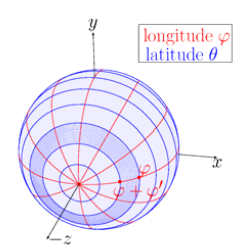
\includegraphics[width=\textwidth]{images/accumulatorarray.png}
        \caption[3D-KHT Accumulator Ball]{}
        \label{fig:accarr}
    \end{subfigure}
    \hspace{\fill}
    \begin{subfigure}{0.25\textwidth}
        \centering
        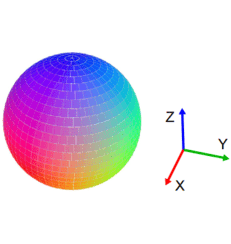
\includegraphics[width=\textwidth]{images/accumulatorball.png}
        \caption[3D-KHT Accumulator Ball]{}
        \label{fig:accball}
    \end{subfigure}
    \hspace{\fill}
    \caption[Hough Transform Accumulators]{Accumulator array (a), taken from \cite*[Figure~3]{Borrmann_Elseberg_Lingemann_Nüchter_2011}. Accumulator
        ball(b) used in 3D-KHT, taken from \cite*[Figure~5]{Limberger_Oliveira_2015}.}
\end{figure}

During the voting procedure, votes are not cast for each data point but rather on previously calculated approximately coplanar clusters.
When casting a vote on a given cluster $c_i$ with its plane (represented by $(\rho, \theta, \phi)$), the corresponding entry in the accumulator ball is updated.
With this update, its neighboring clusters also receive a vote determined by the uncertainty value of $c_i$. Due to the non-discrete
values of uncertainty, the votes are floating-point values as well.

All Peaks within the accumulator ball are detected in the last step. Because the votes tend to be sparsely distributed \cite[Section~3.4]{Limberger_Oliveira_2015},
an auxiliary array $A$ is used to memorize the entries inside the accumulator that are set. When an accumulator index is assigned a value for the first time, it is also added to $A$.
Therefore, it is only necessary to iterate the auxiliary array to find peaks inside the accumulator.
Furthermore, an intermediary smoothing step is performed by merging adjacent peaks inside the accumulator and storing them in $A$.
Then, $A$ is sorted in descending order.
If a cell $c$ in the accumulator has not yet been visited during iteration, $c$ is considered a peak. In addition, $c$ and its 26 neighboring cells are tagged as \textit{visited}.
That way, the most dominant plane, i.e., the one with the most votes, is detected first.
Finally, the detected planes are sorted by the number of different clusters that voted for them.

\subsection{OBRG} \label{sec:bg-obrg}
OBRG (Octree-Based Region Growing \cite{Vo_Truong-Hong_Laefer_Bertolotto_2015}) is also a method that employs region growing.

First, an unorganized point cloud is recursively subdivided using an octree.
An octree node $n$ repeatedly subdivides itself into eight children until the level of $n$ supersedes a predefined maximum subdivision value or if the
amount of contained points in $n$ is less than a predefined minimum of included points.
Saliency features are calculated for every leaf node in preparation for the region growing step. A normal vector is obtained by performing a principle
component analysis (PCA) on the points inside each leaf node. The best-fitting plane of each leaf is defined by the mean normal vector and its center point.
A residual value is obtained by taking the RMS of the distance of all included points to the plane.

For the region growing phase, all leaf nodes are selected as individual seed points. Starting from the seed with the lowest residual value, which relates to a low amount of noise,
a neighboring leaf node $n$ is inserted into the region if $n$ does not belong to any region and the angular divergence between both normal vectors is smaller than
a predefined threshold.

Lastly, a refinement step is employed.
Fast refinement (FR) is performed on regions that succeed in a planarity test, i.e., 70\%-90\% of included points fit the best plane. FR is leaf-based, and all previously unallocated neighboring nodes that satisfy an inlier criterion are added to the region.
General refinement (GR) is performed on regions that are considered non-planar. In contrast to the fast refinement, GR is point based. Therefore,
points from neighboring and previously unallocated leaf nodes are considered and inserted into the region if they, too, satisfy the inlier criterion.
The refinement process returns a complete set of planar regions.

\subsection{PEAC - Probabilistic Agglomerative Hierarchical Clustering}
\subsection{CAPE - Fast Cylinder and Plane Extraction}
\subsection{SCH-RG - Plane Extraction using Spherical Convex Hulls}
\subsection{D-KHT - Hough Transform for Real-Time Plane Detection}
\subsection{DDFF - Depth Dependent Flood Fill}
\subsection{PlaneNet}
\subsection{PlaneRecNet}
\subsection{PlaneRCNN}

\section{Data Formats}
\subsection{Common Input Types}
The fundamental difference between UPC and OPC is their format. Each point cloud has a \textit{width} and a \textit{height} parameter.
An unorganized point cloud $c$ is generally equal to an unordered 1D array of 3D coordinates, i.e., $width = |c|$ and $height=1$.
In contrast, the memory layout of an organized point cloud is a 2D array, where the width and height depend on the resolution of the used sensor.
% T265 kann keine OPC liefern
Taking the maximum resolution of the T265(see Table~\ref{tab:cameraspecs}) as an example, the OPC would have a \textit{width} and \textit{height} of
1280 and 720, respectively.
Intuitively, the value at index (0,0) would be in the top-left corner, and the value at index (\textit{width,height}) would be in the bottom-right corner.
% FIXME bild selber machen: 2xmatrix mit eintrag, einmal (0,0)=XYZ, einmal (0,0) = d_0,0 
Depth images are inherently similar to organized point clouds, given their resolution and two-dimensional structure. The primary difference is that the values
stored in the array are distances to the sensor instead of 3D coordinates.


\section{Datasets}
% FIXME Datensätze erklären
% FIXME Tabelle erläutern!
\begin{table}[]
    \centering
    \begin{tabular}{c|c|c|c|c}
        \textbf{Dataset}                                                                                                                                                                      & \textbf{Input Format} & \textbf{Real} & \textbf{Indoor} & \textbf{GT} \\ \hline
        \textbf{SegComp}     \cite{article}                                                                                                                                                   & DI                    & N             & /               & planes      \\
        \textbf{2D-3D-S}       \cite{armeni_cvpr16}                                                                                                                                           & UPC                   & Y             & Y               & objects     \\
        \textbf{NYU V2}      \cite{10.1007/978-3-642-33715-4_54}                                                                                                                              & DI                    & Y             & Y               & classes     \\
        \textbf{Kinect}      \cite{Oehler_Stueckler_Welle_Schulz_Behnke_2011}                                                                                                                 & OPC                   & Y             & Y               & planes      \\
        \textbf{ICL-NUIM}    \cite{handa:etal:ICRA2014}                                                                                                                                       & DI                    & Y             & Y               & trajectory  \\
        \textbf{SYNBEP}      \cite{schaefer19icra}                                                                                                                                            & OPC                   & N             & /               & planes      \\
        \textbf{ARCO}        \cite{Hidalgo-Paniagua_Vega-Rodríguez_Pavón_Ferruz_2015}                                                                                                         & OPC                   & Y             & Y               & /           \\
        \textbf{SUN}         \cite{7298655}                                                                                                                                                   & DI                    & Y             & Y               & objects     \\
        \textbf{Leica\tablefootnote{\href{https://shop.leica-geosystems.com/de/leica-blk/blk360/dataset-downloads}{https://shop.leica-geosystems.com/de/leica-blk/blk360/dataset-downloads}}} & UPC                   & Y             & N               & planes      \\
        \textbf{TUM}         \cite{sturm12iros}                                                                                                                                               & DI                    & Y             & Y               & trajectory
    \end{tabular}
    \caption[Popular Datasets]{Popular Datasets. The \textit{GT}(Ground Truth) column specifies what the ground truth of each dataset represents.}
    \label{tab:datasets}
\end{table}

\subsection{2D-3D-S}
\subsection{2D-3D-S Experiment}
2D-3D-S was recorded in three different buildings and divided into six distinct areas, including 272 different scenes. A detailed statistic of the included scene types can be found in Table~\ref{tab:stanfordStats}.
An individual scene has a complete unstructured point cloud and a list of annotated files representing semantically different objects that can be found therein.

\textcolor{red}{diese 2 sätze sind dann jetzt wahrscheinlich misplaced}
Furthermore, one could argue that an uneven distribution of scene types introduces a particular bias. While it is true that the distribution is quite uneven, the dataset nevertheless reflects a realistic distribution of scene types since
it is not realistic if a building contains only lecture halls. Inversely, it is appropriate to assume that an office complex contains a substantial amount of hallways needed to connect all offices.

\section{Evaluation Metrics}
Wenn man sachen segmentiert oder muster erkennen möchte usw. benutzt man oft zur evaluierung metriken, die die qualität der benutzten methode beschreiben.
Usual metrics are \textit{precision, recall} and the \textit{f1-score}.
In general, \textit{precision} describes how many of the results are relevant, i.e., the percentage of correctly calculated values(see Eq.~\ref{eq:prec}). \textit{Recall} describes the ratio of relevant results to all relevant data, i.e.
the likelihood of a result being relevant(see Eq.~\ref{eq:rec}). Lastly, the \textit{f1-score} is the harmonic mean of the former two metrics (see Eq.~\ref{eq:f1}).

\begin{equation}
    Precision = \frac{|\{\text{correct values}\} \cap \{\text{obtained values}\}|}{|\{\text{obtained values}\}|}
    \label{eq:prec}
\end{equation}

\begin{equation}
    Recall = \frac{|\{\text{correct values}\} \cap \{\text{obtained values}\}|}{|\{\text{correct values}\}|}
    \label{eq:rec}
\end{equation}

\begin{equation}
    \text{\textit{f1-score}} = 2 \cdot\frac{Precision\cdot Recall}{Precision + Recall}
    \label{eq:f1}
\end{equation}



In the context of this work, we calculate \textit{precision, recall} and the \textit{f1-score} as follows.
Required are the original point cloud $PC$, the corresponding list of ground truth planes $GT$ and the planes obtained from a plane detection algorithm $A$.
First, we regularize the $PC$ to reduce complexity and to avoid proximity bias, because of the inverse relationship
between distance to sensor and cloud density. This regularization is obtained through voxelization of the point cloud.
With this voxel grid, we can now calculate corresponding sets of voxels for each list of points that represent a plane.
In the next step, we compare our planes from $GT$ with $A$ to obtain a list of corresponding pairs of ground truth and found planes.
A ground truth plane $gt_i$ is marked as \textit{detected} if any plane from the list of found planes achieves a minimum voxel overlap of $50\%$.
With this list of correspondences, we calculate \textit{precision, recall} and the \textit{f1-score}.

For a given ground truth plane $gt_j$ and a corresponding detected plane $a_k$ we can sort a given voxel $v_i$ into the categories
\textit{True Positive(TP), False Positive(FP) and False Negative(FN)} as follows.
$$v_i \in gt_j \land v_i \in a_k \Rightarrow v_{i} \in TP$$
$$v_i \in gt_j \land v_i \notin a_k \Rightarrow v_{i} \in FN$$
$$v_i \notin gt_j \land v_i \in a_k \Rightarrow v_{i} \in FP$$
% TODO not needed right? $$v_i \notin gt_j \land v_i \notin a_k \Rightarrow v_{i} \in TN$$  , True Negative(TN)} 

With those four rules, we can calculate the precision, recall and F1 score like this:
$$Precision = \frac{|TP|}{|TP|+|FP|}$$
$$Recall = \frac{|TP|}{|TP|+|FN|}$$

% FIXME ist das hier noch richtig?
Aside from the accuracy, we also need to compare the time each algorithm needs to find its respective set of planes.
For that, we measure the time spent in the plane detection phase, excluding any preprocessing or postprocessing steps.
To measure the detection time, we log the exact times before and after calculations and write the difference to a file.

\end{document}



